\subsection{Cultural variations in polite speech understanding}
\label{sec:culture}

US adults show understanding of polite speech as reflecting epistemic-social tradeoff, whereas children (in our preliminary pilot data) show more subdued inferential patterns, which may be explained in terms of development of polite speech understanding in progress. Now we turn to other populations of interest: different ethnic groups. Different cultures may place different emphases on one of these two communicative goals; some cultures may consider it noble to try to make others feel good by lying, whereas some may regard honesty as the most important virtue. We hypothesize that cultural variations in polite communication arise due to these differences in optimal tradeoff, and the current work will be important first step in testing that hypothesis. 

\subsubsection{Background} 

To the best of our knowledge, there has been no study looking at cross-cultural variations in polite speech understanding in adults. There have been only a few studies that have looked at Chinese and Korean children's ratings of white lies (e.g. \citealt{fu2007, ma2011}). For example, Chinese children as young as 7 years rate lie-telling as positive in a public than private situation, and as negative when accurate information would help the listener \citep{ma2011}. But these studies do not offer comparisons with European American children (cf. \citealt{lee1997}). In our proposed work, we hope to directly compare three groups of interest, for both adults and children: US, India, and South Korea. These areas cover a wide range of languages used, religions and socioeconomic statuses, and thus will help provide a comprehensive view over the general trend of pragmatic language understanding across different cultures.


\subsubsection{Empirical tests}


{\bf Experiment 4: Indian and Korean adults' true state inference.} 
This experiment will be identical in structure as Experiment 1, and they will reason about the true state given speaker's utterance and goal. Indian participants will be recruited on Amazon's Mechanical Turk, and Korean participants by advertising on Facebook. Participants will be recruited in two batches: one that speaks Hindi and the other that speaks English; and we will compare the data to examine any differences that may arise from language.  

{\bf Experiment 5: Indian and Korean adults' goal inference.} 
This experiment will be identical in structure as Experiment 2, and they will reason about the true state given speaker's utterance and goal. Participants will be recruited in an identical manner to Experiment 4.

{\bf Experiment 6: US, Indian and Korean adults' joint inference over true state and goal.} 
Additionally, we will test adults' joint inferences over true state and goals given an utterance across all sites. By providing no information on true state or speaker's goals, this experiment will be a useful test for determining people's lay expectations for a speaker's goals (to be honest versus nice). Participants will be recruited in an identical manner to Experiment 4.

{\bf Experiment 7: Indian and Korean children's understanding of polite speech.} 
This experiment will be identical in structure as Experiment 3. Participants will be recruited at elementary schools in India and South Korea. Across these three different sites, we will recruit three different age groups (3-4, 5-6 and 7-8-year-olds), with a minimum of 10 and maximum of 24 participants per condition, age group and site, allowed by the total testing time at the field sites. They will be tested in English or their native language (Korean, Hindi or Gujarati), with a script that is directly translated from English by an educated native speaker. Those who are not exposed to the language of instruction at least 75\% daily will be excluded from data analysis. Adult participants (60 for each site and condition) will be recruited on Amazon's Mechanical Turk, and will be asked to participate in an online version of the child study to be examined as controls.

\subsubsection{Results from pilot work (Experiment 7)} 

Figure~\ref{fig:expt4} shows an example analysis conducted on pilot data. Whereas US children attributed more niceness to polite speaker compared to honest speaker increasingly with age, Indian children showed the opposite trend of attributing more niceness to honest than polite speaker across both age groups. This is preliminary yet promising evidence that construal of niceness (linked to the notion of optimal tradeoff of truthfulness versus face-saving) may be different across cultures. We will seek to verify this trend with larger sample sizes to account for variability and ensure robustness of judgment patterns.

\begin{figure*}[t]
\begin{centering}
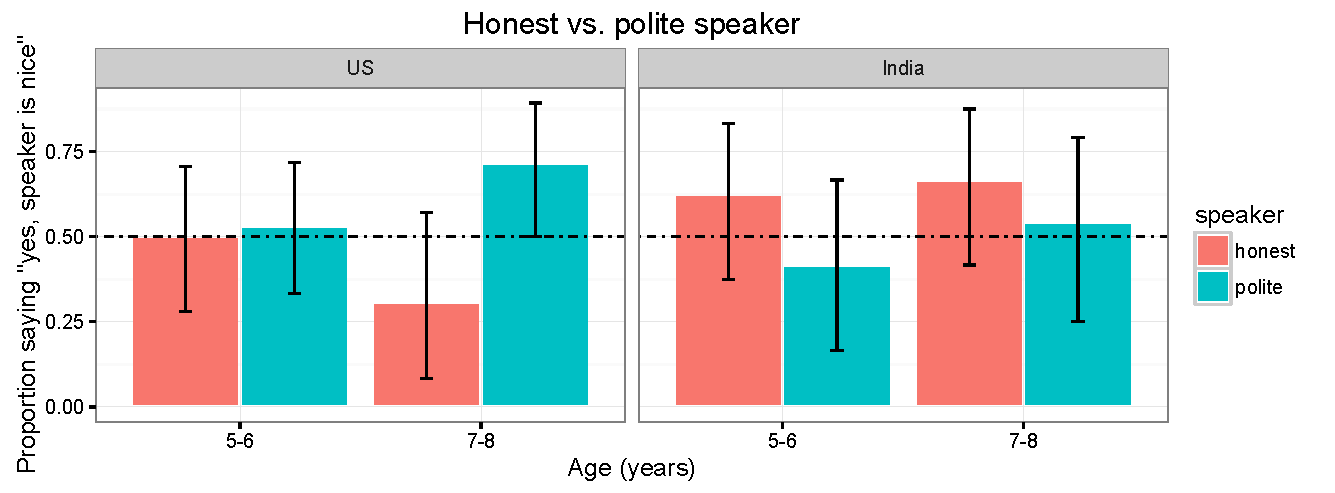
\includegraphics[width=\textwidth]{figures/exp4.pdf}
\caption{\label{fig:expt4} Results from Experiment 7 (pilot), for US versus Indian children's niceness judgments for honest versus polite (but dishonest) speaker. Error bars represent 95\% confidence intervals.}
\end{centering}
\end{figure*}

\subsubsection{Implications for the model}

Preliminary data from Indian child participants show an interesting reversal in speaker niceness attribution: Indian children tend to say that an honest speaker is more ``nice'' than a polite speaker. In light of our model, two interpretations are possible (if the patterns hold up): either Indian children do not reason about polite language based on epistemic-social tradeoff as we hypothesized, or Indian children have a different construal of the word ``nice,'' to mean ``optimal'' rather than ``kind'' or ``caring''. Is the latter is true, then it informs that language of instruction is a critical consideration in conducting these studies, and that Indians may have a different sense of what comprises an ``optimal'' communication from the US population. Our proposed work addresses both of these issues, in that we will conduct each Experiment at each site in two languages: the local language and English, to look at any differences in responses that are caused by language rather than cultural differences; and we will inquire what each cultural group thinks of as an optimal, cooperative speaker.


%%% Local Variables: 
%%% mode: latex
%%% TeX-master: "desc"
%%% End

